\chapter{Drogues}
\label{sec:drogues}

During a hydrodynamic simulation, \telemac{3D} offers an opportunity to follow
the paths of a number of particles (drogues) which are released into the fluid
from discharge points. The result is provided in the form of a
TECPLOT-formatted file which contains the various positions of the drogues.


\section{Configuration of simulation}

three parameters should be entered into the steering file. First, the user
should mention the number of drogues by means of the keywords \telkey{NUMBER OF
DROGUES}, the default value of which is 0. Secondly, the user should enter the
name of the file into which \telemac{3D} will store the successive positions of
the drogues. This is defined through the keyword \telkey{DROGUES FILE}. Lastly,
the user can configure the printout period within that file by means of the
keyword \telkey{PRINTOUT PERIOD FOR DROGUES} (default value = 1). That value is
expressed in a number of time steps and is quite independent from of the
printout period of the other results in \telemac{3D}.

The subroutine \telfile{ADD\_PARTICLE} is called within the \telfile{FLOT3D}
subroutine to set the initial values of variables \telfile{XFLOT, YFLOT, ZFLOT}
and \telfile{TAGFLO}, which are the three-dimensional coordinates of the
release point and an identifier of the particle for each drogue.
The release time step is also to be amended.
A commented example can be found within the subroutine \telfile{FLOT3D} or
in the example ``particles''.
This subroutine is to be inserted in the FORTRAN file.

The example below illustrates the programming of the steering file in the case
of two drogues being release at different times.

\begin{lstlisting}[language=TelemacCas]
NUMBER OF DROGUES                   = 2
DROGUES FILE                        = './drogues'
PRINTOUT PERIOD FOR DROGUES         = 10
\end{lstlisting}

\section{Visualisation of results}
\label{sec:droguesfile}
the results are stored in the file specified by the keyword \telkey{DROGUES
FILE}. This is an ASCII file written in a format compatible with
the TECPLOT software. If this tool is not available, it is quite easy to get
the coordinates of the different drogue positions to export them to another
viewer. It is also possible to develop a new drogue output format, but this
must be done in the subroutine \telfile{DERIVE}.

Within TECPLOT, in order to add the Tecplot \telkey{DROGUES FILE} to TELEMAC
result data already loaded, select ``Add to current data'' set in the
\textbf{Load Data File Warning dialogue} (cf. Figure \ref{fig:load_data}). The
Load Data File Warning dialogue will appear after the user has selected the
file and zones and/or variables to load.

\begin{figure}[H]%
\begin{center}
%
  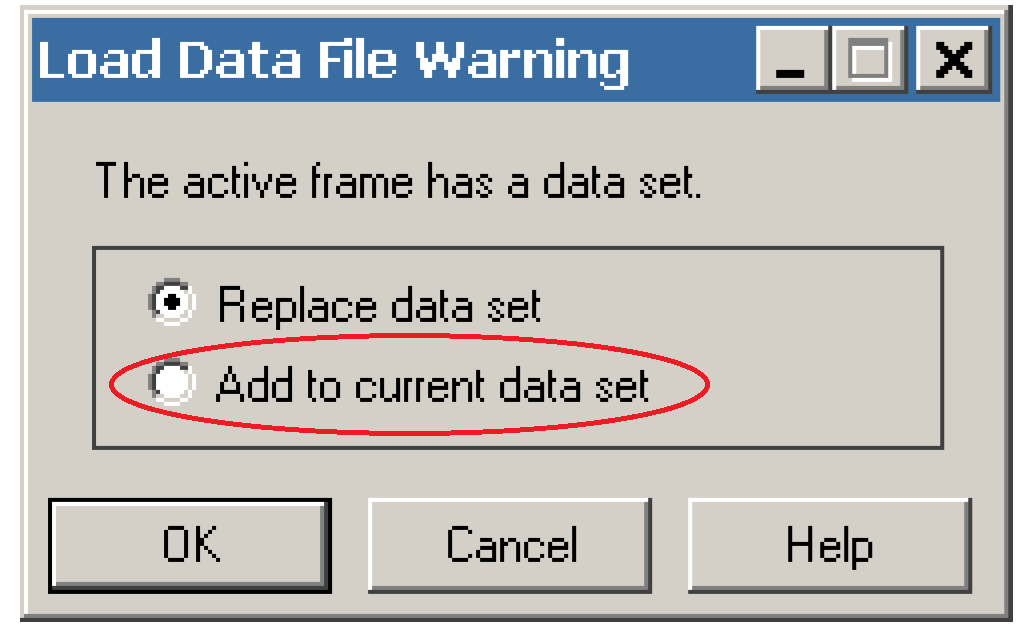
\includegraphics[width=0.6\textwidth]{./graphics/load_data}
%
\end{center}
\caption
[Load Data File Warning dialogue in TECPLOT]
{Load Data File Warning dialogue in TECPLOT.}
\label{fig:load_data}
\end{figure}

Once you have loaded your data with TECPLOT, the drogue positions will be
considered as ``Scatter plots'' by Tecplot Software. Scatter plots are plots of
symbols centered at the data points in a field. To add a scatter layer to your
plot, activate the ``Scatter'' toggle in the Sidebar. To be visible in your
plot, the Scatter layer which contains the Tecplot \telkey{DROGUES
FILE} must be turned on and the Scatter layer containing the \telkey{3D RESULT
FILE} data must be turned off. This is done by selecting ``Yes'' or ``No'' from
the [Scat Show] button drop-down menu on the Scatter page of the \textbf{Zone
Style dialogue} (cf. Figure \ref{fig:zone_style}).

\begin{figure}[H]%
\begin{center}
%
  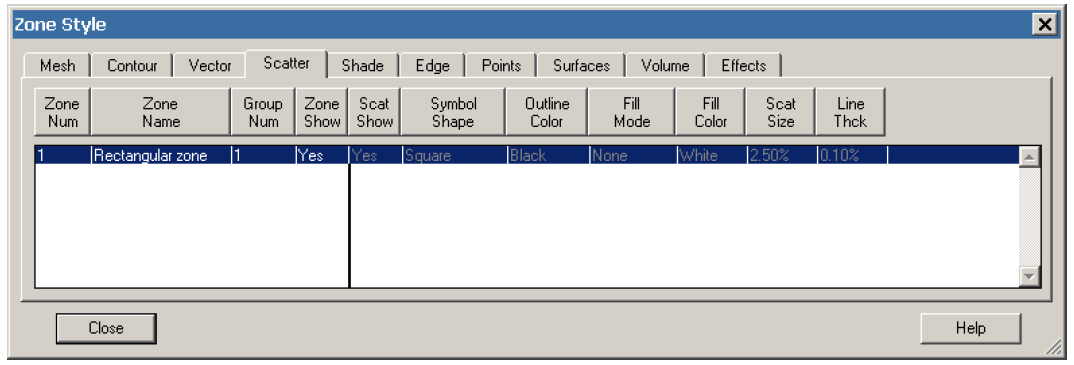
\includegraphics[width=0.7\textwidth]{./graphics/zone_style}
%
\end{center}
\caption
[Zone Style dialogue in TECPLOT]
{Zone Style dialogue in TECPLOT.}
\label{fig:zone_style}
\end{figure}

Then, you can modify your Scatter plot using the Scatter page of the
\textbf{Zone Style dialogue} and the Scatter submenu of the \textbf{Plot menu}.
You can control any of the following attributes for a zone or group of zones
from the Scatter page of the Zone Style dialogue. For complementary information
on the Tecplot procedure, the reader may refer to the Tecplot user guide.
